\subsection{Estados cuánticos y el término Qubit}
En física cuántica, el estado cuántico es cualquier estado posible en el que puede estar un sistema mecánico cuántico. Un estado cuántico completamente especificado puede describirse mediante un vector de estado, una función de onda o un conjunto completo de números cuánticos para un sistema específico. Un estado cuántico parcialmente conocido, como un conjunto con algunos números cuánticos fijos, puede ser descrito por un operador de densidad.\\\\
Una mezcla de estados cuánticos es nuevamente un estado cuántico. Los estados cuánticos que no se pueden escribir como una mezcla de otros estados se denominan estados cuánticos puros, mientras que todos los demás estados se denominan estados cuánticos mixtos. Un estado cuántico puro se puede representar mediante un rayo en un espacio de Hilbert sobre los números complejos, mientras que los estados mixtos se representan mediante matrices de densidad, que son operadores semidefinitos positivos que actúan en el espacio de Hilbert.\\\\
Un bit cuántico, qbit o qubit es la unidad básica de información cuántica, es la versión cuántica del clásico bit binario.
\subsection{Puertas lógicas clásicas y cuánticas}
\subsection{Operador de Hadamart}
\subsubsection{Transformada de Fourier clásica y cuántica}
\subsection{Algoritmo de Shor}
\subsubsection{Periodo de la función a\textsuperscript{x}mod N}
Se tiene la función \begin{equation}
    f(x)=a^x mod N
    \label{eq:axmodn}
\end{equation}
donde $a$ y $N$ son enteros positivos tal que $a<N$ y que no tienen ningún factor en común. El periodo (o el orden r), es el valor más pequeño 
diferente de cero tal que:
\begin{equation}
    a^r mod N =1
    \label{eq:condicionr}
\end{equation}
Usando como ejemplos $a=3$ y $N=35$, se tiene el siguiente periodo:
\begin{figure}[H]
    \centering
    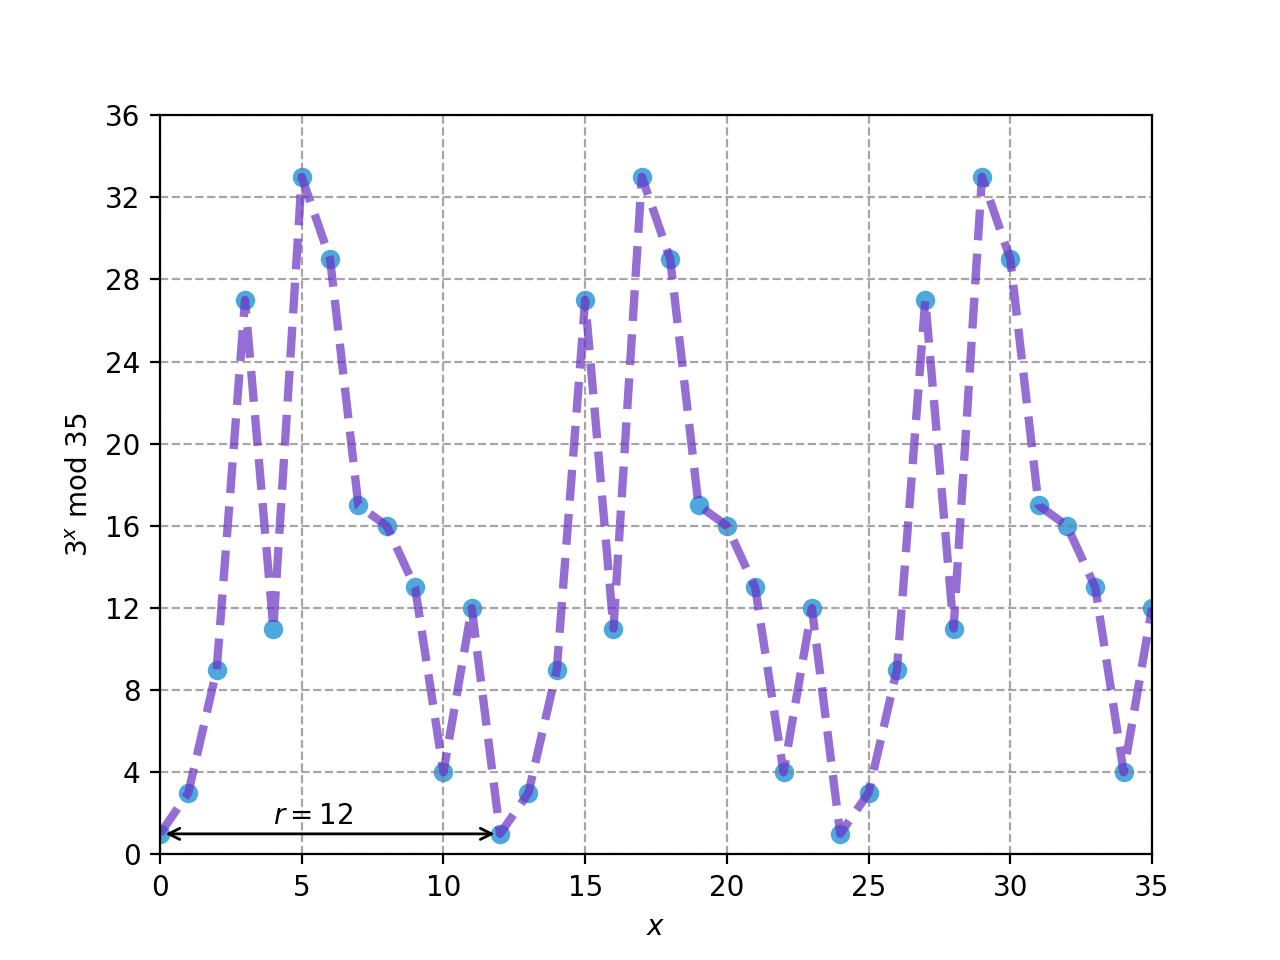
\includegraphics[scale=0.65]{../Graphics/period.png}
    \caption{Periodo de la función \ref{eq:axmodn} para visualizar la condición \ref{eq:condicionr} usando el código \ref{cod:rperiod}}
    \label{fig:condicionr}
\end{figure}
Para realizar esta operación dentro del Algoritmo de Shor se propusó un operador unitario tal que:
\begin{equation}
    U \left| y \right\rangle \equiv \left| ay mod N \right\rangle 
    \label{eq:umod}
\end{equation}
Para visualizar el funcionamiento de este operador se usará el ejemplo de $a=3$ y $N=35$, trabajando con los eigenestados de U empezando con el estado 
$\left|1\right\rangle$ podemos visualizar que la transformación sucesiva del operador U estariasmos multiplicando el estado por $amodN$, por lo tanto, después de
r transformaciones regresaremos al estado $\left|1\right\rangle$.
\begin{align*}
    U\left| 1 \right\rangle &= \left|3\right\rangle \\
    U^2\left| 1 \right\rangle &= \left|9\right\rangle \\
    U^3\left| 1 \right\rangle &= \left|12\right\rangle \\ 
                    & \vdots  \\ 
    U^{r-1}\left| 1 \right\rangle &= \left|12\right\rangle \\
    U^r\left| 1 \right\rangle &= \left|1\right\rangle \\
\end{align*}
Utilizando una superposición de estos estados, obtendremos lo siguiente:
\begin{equation}
    \left| u_0 \right\rangle = \frac{1}{\sqrt{r}} \sum\limits_{k=0}^{r-1} \left|a^k mod N \right\rangle.
    \label{eq:u0}
\end{equation}
Realizando esa serie para $a=3$ y $N=35$, encontramos que el estado descrito en \ref{eq:uo} es invariante bajo la transformación de U.
\begin{align*}
    \left| u_0 \right\rangle &= \frac{1}{\sqrt{12}} \left(\left|1\right\rangle + \left|3\right\rangle+ \left|9\right\rangle 
    +\cdots +\left|4\right\rangle + \left|12\right\rangle \right)\\
    U\left| u_0 \right\rangle &= \frac{1}{\sqrt{12}} \left(U\left|1\right\rangle + U\left|3\right\rangle+ U\left|9\right\rangle 
    +\cdots +U\left|4\right\rangle + U\left|12\right\rangle \right)\\
    &= \frac{1}{\sqrt{12}} \left(\left|3\right\rangle + \left|9\right\rangle+ \left|27\right\rangle 
    +\cdots +\left|12\right\rangle + \left|1\right\rangle \right)\\
    &= \left| u_0 \right\rangle .
\end{align*}
Lo cual obtenemos que el eigenvalor es 1. Un eigenestado más general es aquel el cual contenga una fase diferente para cada base de estados. Especificamente, veremos el caso
donde cada fase del k-esimo es proporcional a k, de tal manera que:
\begin{align}
    \label{eq:u1}
    \left| u_1 \right\rangle &= \frac{1}{\sqrt{r}} \sum\limits_{k=0}^{r-1} e^{-\frac{2\pi i k}{r}} \left| a^k mod N \right\rangle \\
    \label{eq:ua1}
    U\left| u_1 \right\rangle &= e^{\frac{2\pi i}{r}} \left| u_1 \right\rangle.
\end{align}
Teniendo así un único eigenestado para cada valor entero en $s$ donde $0\leq s \leq r-1 $
\subsection{Implementación con Qiskit}